\subsection{Reset DCB master GBTx}
A hardware reset can be performed on the master FFC breakout board to reset the
master GBTx (See \autoref{fig:dcb_mc_reset}).

\begin{figure}[!ht]
\centering
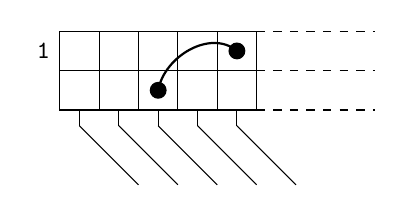
\begin{tikzpicture}
    % Pins
    \draw (0,0) rectangle (0.5,0.5);
    \draw (0.5,0) rectangle (1,0.5);
    \draw (1,0) rectangle (1.5,0.5);
    \draw (1.5,0) rectangle (2,0.5);
    \draw (2,0) rectangle (2.5,0.5);

    \draw (0,-0.5) rectangle (0.5,0);
    \draw (0.5,-0.5) rectangle (1,0);
    \draw (1,-0.5) rectangle (1.5,0);
    \draw (1.5,-0.5) rectangle (2,0);
    \draw (2,-0.5) rectangle (2.5,0);

    % Extension lines
    \draw [dashed] (2.5,0.5) -- (4,0.5);
    \draw [dashed] (2.5,0) -- (4,0);
    \draw [dashed] (2.5,-0.5) -- (4,-0.5);

    % Additional copper traces
    \draw (0.25,-0.5) -- (0.25,-0.7);
    \draw (0.75,-0.5) -- (0.75,-0.7);
    \draw (1.25,-0.5) -- (1.25,-0.7);
    \draw (1.75,-0.5) -- (1.75,-0.7);
    \draw (2.25,-0.5) -- (2.25,-0.7);

    \draw (0.25,-0.7) -- (1,-1.45);
    \draw (0.75,-0.7) -- (1.5,-1.45);
    \draw (1.25,-0.7) -- (2,-1.45);
    \draw (1.75,-0.7) -- (2.5,-1.45);
    \draw (2.25,-0.7) -- (3,-1.45);

    % Helper labels (imaginary)
    \coordinate (B) at (0,0.25);
    \node at (B) [left] {\small\texttt{1}};

    % GND
    \draw [black,fill] (2.25,0.25) circle [radius=0.1];

    % RESET
    \draw [black,fill] (1.25,-0.25) circle [radius=0.1];

    % Connect GND and RESET
    \draw [thick] (1.25,-0.25) to [out=80,in=140] (2.25,0.25) node {};
\end{tikzpicture}
\caption{
    Connect the two pins marked above with a jumper/wire to reset DCB master
    GBTx.
    Note that pin 7 and 9 are both \texttt{GND}.
}
\label{fig:dcb_mc_reset}
\end{figure}
